%BEGIN TICKET 14
\begin{definition}
    Пусть есть $[a, b]$. Тогда дробление (разбиение, пунктир) отрезка: набор точек:  $x_0 = a < x_1 < x_2 < \ldots < x_n = b$.
\end{definition}
\begin{definition}
    Ранг дробления: $\max\limits_{k=1,2,\ldots, n}(x_k - x_{k-1}) \eqqcolon |\tau|$, $\tau = (x_0, x_1, \ldots, x_n)$
\end{definition}

\begin{definition}
    Оснащение дробления --- набор точек $\xi = ( \xi_1, \xi_2, \ldots, \xi_n)$, такой что $\xi_k \in [x_{k-1}, x_k]$.
\end{definition}
\begin{definition}
    Интегральная сумма (сумма Римана) $S(f, \tau, \xi) \coloneqq = \sum\limits_{k=1}^n f(\xi_k)(x_k - x_{k-1})$, 

    \textit{По факту просто сумма площадей прямоугольников под графиком}
    \begin{figure}[h!]
    	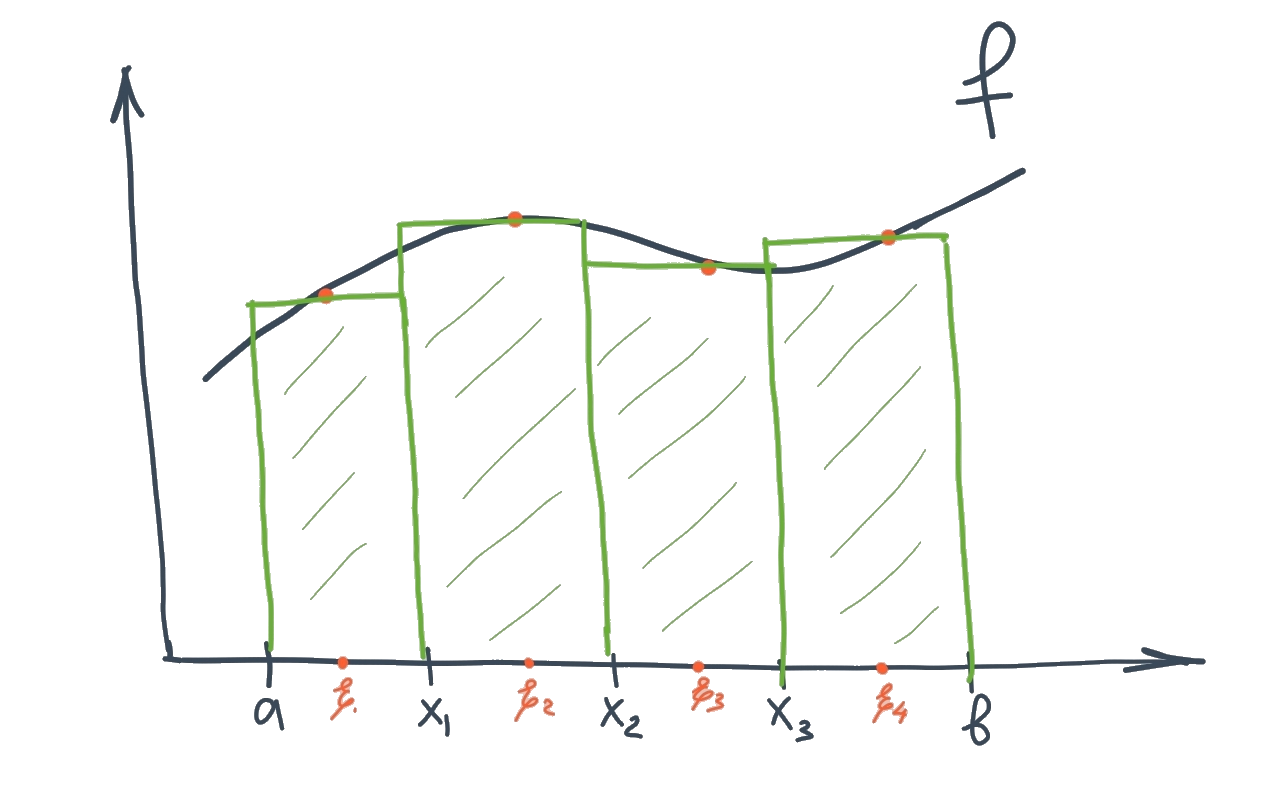
\includegraphics[scale=0.2]{riemann_sum}
    \end{figure}
\end{definition}
%END TICKET 14